\section{Model Architecture Design}

Python and Jupyter notebooks were used to implement the models and train them on the plant seedlings dataset. The code was organized into separate notebooks for each model, allowing for easy experimentation and comparison of different architectures. Libraries such as PyTorch, Scikit-learn, NumPy and Pandas were used for data manipulation, model training and evaluation.

To achieve deterministic results and reproducibility, the random seed \textit{42} was set at the beginning of each notebook. This ensured that the same random initialization was used for each run, leading to consistent results across different experiments:

\begin{minipage}{0.9\linewidth}\begin{lstlisting}[caption={Settings to achieve deterministic results and ensure reproducibility.},label={lst:deterministic-results}]
RANDOM_SEED = 42

seed(RANDOM_SEED)
np.random.seed(RANDOM_SEED)

torch.manual_seed(RANDOM_SEED)
torch.cuda.manual_seed_all(RANDOM_SEED)

torch.backends.cudnn.deterministic = True
torch.backends.cudnn.benchmark = False
\end{lstlisting}\end{minipage}

The random seed was set for the Python, NumPy and PyTorch random number generator. Additionally, the cuDNN backend was set to deterministic mode to ensure that the results are reproducible on the GPU.

\subsection{Guessing Baseline}

As a starting point and to get familiar with the dataset and the Kaggle competition, a simple guessing baseline was implemented. The baseline assigns the most frequent class label to all test samples. This approach provided a lower bound on model performance and served as a reference point for evaluating the effectiveness of more sophisticated models. The head of the submission file is shown below:

\begin{minipage}{0.9\linewidth}\begin{lstlisting}[language={},caption={Head of guessing baseline submission file.},label={lst:guessing-baseline}]
file,species
1b490196c.png,Loose Silky-bent
85431c075.png,Loose Silky-bent
506347cfe.png,Loose Silky-bent
7f46a71db.png,Loose Silky-bent
668c1007c.png,Loose Silky-bent
...
\end{lstlisting}\end{minipage}

In this case, all \textit{794} test samples were assigned the class label ``Loose Silky-bent'', which is the most frequent class in the training dataset. The F1-score of this baseline is \textbf{0.14105}.

\subsection{Custom CNN}

The custom CNN architecture was designed (from scratch) to capture features relevant to seedling classification, while being lightweight enough to be effectively trained locally on the given dataset. The model consists of a series of convolutional and pooling layers followed by fully connected layers to learn features hierarchically and make the final class prediction.

\begin{figure}[htbp]
    \centerline{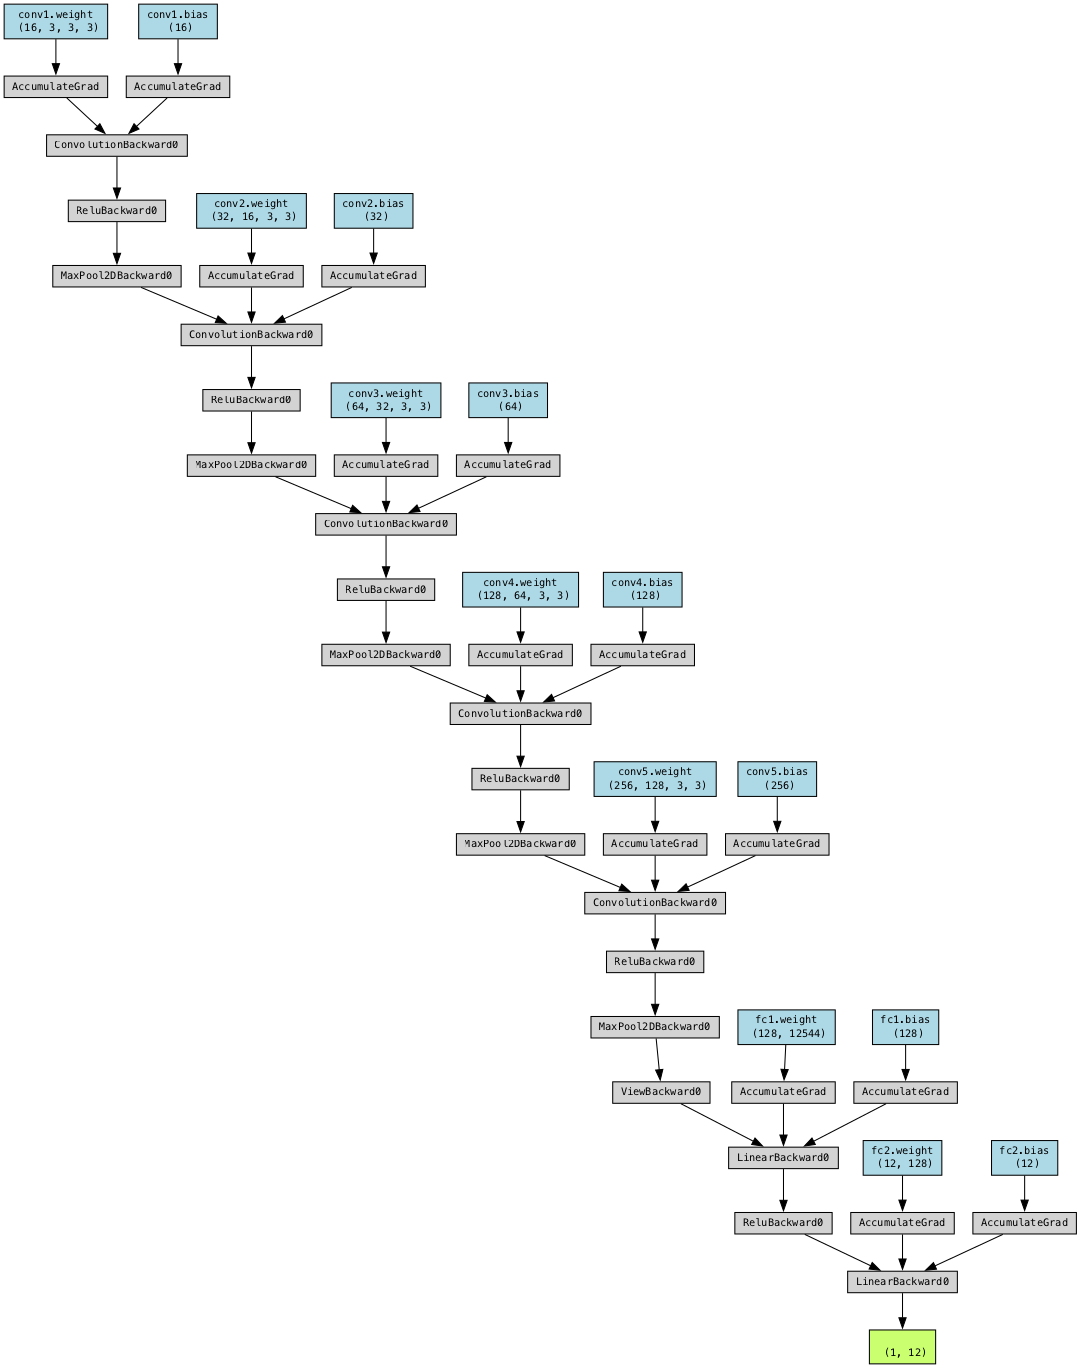
\includegraphics[width=0.9\linewidth]{../../resources/custom_cnn/architecture.png}}
    \caption{Custom CNN architecture, consisting of convolutional and pooling layers followed by fully connected layers.}
    \label{fig:custom-cnn-architecture}
\end{figure}

As shown in Fig.~\ref{fig:custom-cnn-architecture}, the network begins with a series of convolutional layers~(blue), with the number of filters gradually increasing from \textit{16} to \textit{256}. These convolutional layers, each followed by a Rectified Linear Unit~(ReLU) activation, extract spatial features such as edges, textures and patterns from the images. To reduce spatial dimensions and computational complexity, max-pooling layers~(gray) are applied after each convolutional block to focus on the most salient features.

After the convolutional and pooling stages, the feature maps are flattened into a 1D vector that serves as the input to the fully connected layers~(blue). The first fully connected layer has \textit{128} neurons and captures high-level abstract features, while the final fully connected layer maps these features to the \textit{12} target classes~(green), producing the class probabilities.

The final custom CNN model has approximately \textit{2 million} parameters, making it lightweight and computationally efficient compared to the following architectures. The model architecture is designed to capture relevant features for seedling classification while being suitable for training on a moderate-sized dataset.

\subsection{Pre-trained CNN}

As an alternative to training and building a custom CNN from scratch, a pre-trained CNN can be used to leverage learned features from a large dataset. The pre-trained model ResNet-18~\cite{DBLP:journals/corr/HeZRS15} was used as a feature extractor, where the final classification layer was replaced with a new fully connected layer to predict the \textit{12} plant seedling classes:

\begin{minipage}{0.9\linewidth}\begin{lstlisting}[caption={Replacing the final classification layer of a pre-trained ResNet-18 model.},label={lst:pre-trained-cnn}]
from torchvision import models
from torch.nn import Linear

model = models.resnet18(
    weights=models.ResNet18_Weights.DEFAULT
)
model.fc = Linear(
    in_features=model.fc.in_features,
    out_features=len(dataset.classes),
)
\end{lstlisting}\end{minipage}

The \texttt{ResNet18} model has been pre-trained on the ImageNet dataset~\cite{5206848ImageNet} and has shown strong performance on a variety of computer vision tasks~\cite{DBLP:journals/corr/HeZRS15}. By using a pre-trained model, the network can leverage the learned features from ImageNet to improve performance on the plant seedlings dataset. The final classification layer was replaced to adapt the model to the specific classification task.

This pre-trained CNN model has approximately \textit{11 million} parameters, making it deeper than the custom CNN. However, fine-tuning the weights allow the model to learn more complex features and hopefully achieve better performance on the plant seedlings dataset.

\subsection{Pre-trained ViT}

Another approach is to use a ViT as the backbone architecture. The ViT model has been pre-trained on \mbox{ImageNet-21k}~\cite{ridnik2021imagenet}~(including plants/crops) and then fine-tuned~\cite{steiner2021train} on the plant seedlings dataset. The final classification head was replaced with a new linear layer to predict the \textit{12} plant seedling classes:

\begin{minipage}{0.9\linewidth}\begin{lstlisting}[caption={Replacing the final classification layer of a pre-trained ViT model.},label={lst:pre-trained-vit}]
import timm
import torch

model = timm.create_model(
    "vit_base_patch16_224",
    pretrained=True,
    num_classes=num_classes
)
model.head = torch.nn.Linear(
    model.head.in_features,
    num_classes
)
\end{lstlisting}\end{minipage}

Instead of fine-tuning the entire model, the pre-trained weights of the \texttt{vit\_base\_patch16\_224} model~\cite{Wightman_PyTorch_Image_Models} were frozen and only the classification head was trained on the plant seedlings dataset. Transfer learning leverages the powerful feature extraction capabilities of the pre-trained model while adapting the final layer to the specific classification task~\cite[Chapter~6]{bishop2024deep}. Furthermore the computational cost is reduced compared to training the entire model from scratch or fine-tuning all layers:

\begin{minipage}{0.9\linewidth}\begin{lstlisting}[caption={Freezing the pre-trained ViT backbone and training only the classification head.},label={lst:freeze-vit-backbone}]
for param in model.parameters():
    param.requires_grad = False

for param in model.head.parameters():
    param.requires_grad = True
\end{lstlisting}\end{minipage}

The ViT model has approximately \textit{86 million} parameters, but only \textit{9,228} of these are adapted in the experiments. This makes the model computationally efficient, while still benefiting from the powerful feature extraction capabilities of the pre-trained ViT model.

\subsection{Ensemble}

Several challenges have shown that an ensemble of models can often outperform individual models, especially when inference time is not a primary concern~\cite{Stallkamp2012,DBLP:journals/corr/HeZRS15}. A final ensemble was created by combining the predictions of all three models (custom CNN, pre-trained CNN, pre-trained ViT) using a weighted average. The weights were determined based on the performance of each model on the test set:

\begin{minipage}{0.9\linewidth}\begin{lstlisting}[caption={Ensemble predictions using a weighted average.},label={lst:ensemble}]
import torch.nn.functional as F

model_custom_cnn.eval()
model_resnet.eval()
model_vit.eval()

w_custom_cnn = 0.25
w_resnet = 0.25
w_vit = 1 - w_custom_cnn - w_resnet

...

probs_custom_cnn = (
    F.softmax(model_custom_cnn(images), dim=1)
)
probs_resnet = (
    F.softmax(model_resnet(images), dim=1)
)
probs_vit = (
    F.softmax(model_vit(images), dim=1)
)

probs_ensemble = (
    w_custom_cnn * probs_custom_cnn +
        w_resnet * probs_resnet +
            w_vit * probs_vit
)

_, preds = torch.max(probs_ensemble, 1)
\end{lstlisting}\end{minipage}

The ensemble combines the strengths of each individual model to improve overall performance and robustness. By averaging the predictions of multiple models, the ensemble can reduce the impact of individual model weaknesses and provide more reliable predictions (\textit{wisdom of the crowd}~\cite[Chapter~7]{geronoctober2022hands}). As the ViT model achieved the highest performance on the test set, it is assigned the highest weight in the ensemble (\textit{0.5}), while the custom CNN and ResNet models are assigned equal weights (both \textit{0.25}).

\subsection{Summary}

\begin{table}[htbp]
    \caption{Model parameters and size of the custom CNN, pre-trained CNN and pre-trained ViT.}
    \begin{center}
        \resizebox{0.9\linewidth}{!}{
            \begin{tabular}{|c|c|c|c|}
                \hline
                \textbf{Model}  & \textbf{Total Params} & \textbf{Trainable Params} & \textbf{Total Size (MB)} \\
                \hline
                Custom CNN      & 1,999,916             & 1,999,916                 & 34.91                    \\
                \hline
                Pre-trained CNN & 11,182,668            & 11,182,668                & 106.02                   \\
                \hline
                Pre-trained ViT & 85,655,820            & 9,228                     & 806.35                   \\
                \hline
            \end{tabular}
            \label{tab:parameters}
        }
    \end{center}
\end{table}

Table~\ref{tab:parameters} shows the total number of parameters and the size of each model. The custom CNN has the smallest number of parameters and size, making it lightweight and computationally efficient. The pre-trained CNN has a larger number of parameters, while the pre-trained ViT has the largest, but only a small fraction of them are trainable during the experiments. This allows for efficient training while still benefiting from the powerful feature extraction capabilities of the pre-trained model.